\documentclass[times, utf8, diplomski]{fer}
\usepackage{booktabs}
\usepackage[final]{pdfpages}
\usepackage{listings}
\usepackage{keyval}


\lstdefinelanguage{Javascript}{
  keywords={typeof, new, true, false, catch, function, return, null, catch, switch, var, if, in, while, do, else, case, break, let, const},
  keywordstyle=\color{black}\bfseries,
  ndkeywords={class, export, boolean, throw, implements, import, this},
  ndkeywordstyle=\color{black}\bfseries,
  identifierstyle=\color{black},
  sensitive=false,
  comment=[l]{//},
  morecomment=[s]{/*}{*/},
  commentstyle=\color{black}\ttfamily,
  stringstyle=\color{red}\ttfamily,
  morestring=[b]',
  morestring=[b]"
}

\lstset{
   language=JavaScript,
   backgroundcolor=\color{white},
   extendedchars=true,
   basicstyle=\footnotesize\ttfamily,
   showstringspaces=false,
   showspaces=false,
   numbers=left,
   numberstyle=\footnotesize,
   numbersep=9pt,
   tabsize=2,
   breaklines=true,
   showtabs=false,
   captionpos=b
}

\renewcommand\lstlistingname{Isječak koda}
\renewcommand\lstlistlistingname{Popis isječaka koda}

\nocite{*}

\begin{document}
% TODO: Navedite broj rada.
\thesisnumber{2345}

\title{Proceduralno generiranje trave i niskog raslinja}
\author{Mihael Međan}

\maketitle

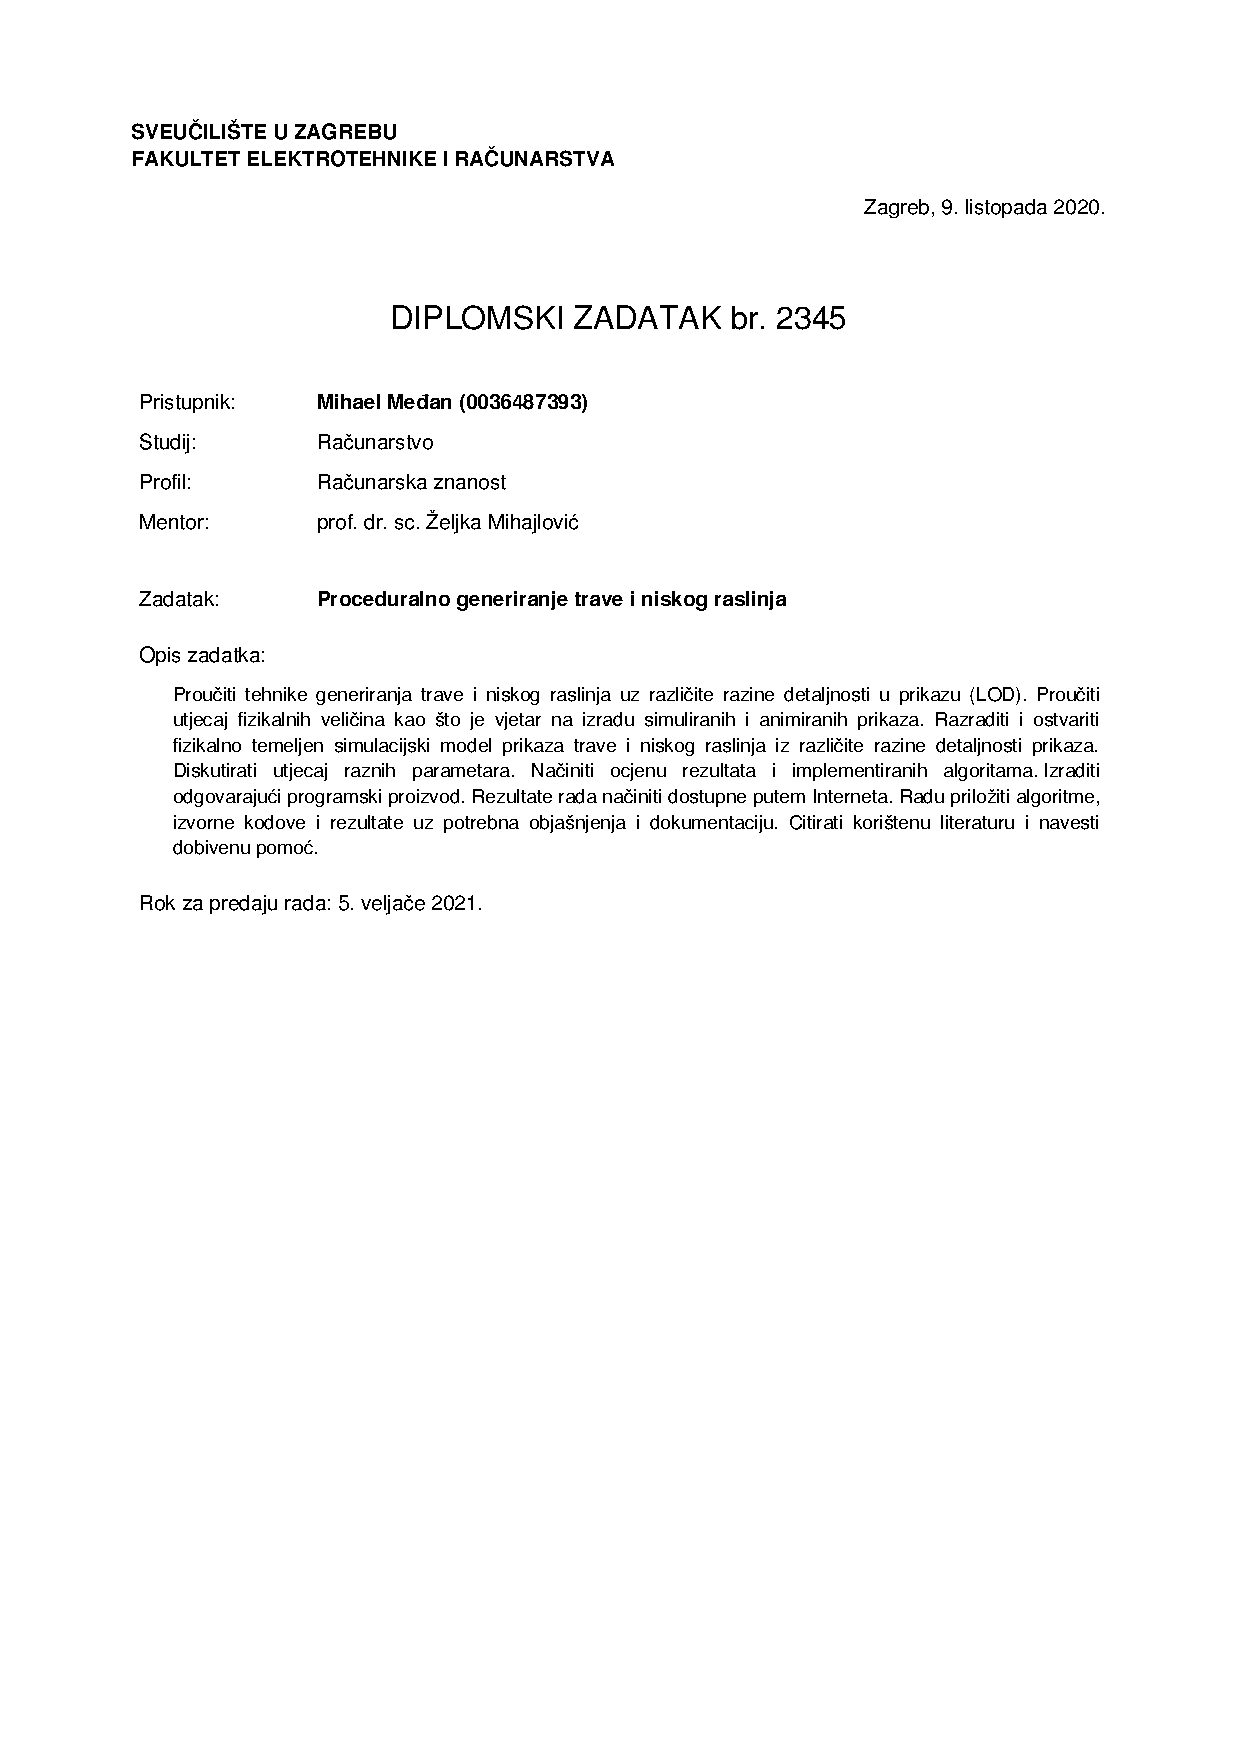
\includepdf[pages=-,offset=0 -75]{hr_0036487393_56.pdf}

\zahvala{}

\tableofcontents

\chapter{Uvod}
\paragraph{}
Proceduralno generiranje 3D modela je izrazito široko područje s velikim brojem različitih 
pristupa rješavanju tog problema ovisno o primjeni. Generiranje modela se u novije vrijeme 
sve češće radi skeniranjem stvarnih objekata. Ovakav način generiranja modela daje 
impresivne rezultate, ali takvi rezultati su često izrazito kompleksni s jako puno 
geometrije i neupotrebljivi su u interaktivnim sustavima poput video igara. 

\paragraph{}
U video igrama je potreban minimalan broj detalja kako bi brzina izvođenja aplikacije bila 
što veća, ali dovoljno velik da daje dojam stvarnosti. Današnje igre sve više teže prema 
otvorenom svijetu (engl. \textit{open-world}). Kod takvih igara igraču je prepuštena potpuna 
sloboda kretanja na velikim površinama. Sa željom da povećaju brzinu izvođenja, programeri 
koriste tehniku iscrtavanja prikaza s različitom razinom detalja. Kod ovakvog pristupa, 
objekti koji su daleko od kamere koriste modele s izrazito malo detalja, a kod objekata 
koji su bliže kameri koriste detaljne modele. Budući da su modeli koji su udaljeni od kamere 
na ekranu mali, igrač ne može vidjeti gubitak detalja i dojam stvarnosti mu ostaje velik.

\paragraph{}
Još jedan od problema koji se susreće kod igara s otvorenim svijetom je vegetacija. Pojedine 
lokacije igrinog svijeta imaju potpuno različite vegetacije. Ovo iziskuje vrlo velik napor 
od umjetnika koji moraju modelirati različite vegetacije za različite lokacije. Osim velikog 
broja različitih biljaka, zbog tehnike iscrtavanja u različitoj razini detalja često je za 
isti model potrebno napraviti nekoliko različitih modela s različitom razinom detalja, što 
dodatno rezultira vremenom potrebnim za izradu igre. Igre su interaktivni sustav i statični 
objekti koji su u stvarnom svijetu dinamički razbijaju osjećaj stvarnosti. Zbog toga je sve 
te modele potrebno i animirati.

\paragraph{}
Kroz ovaj rad istražena je tehnika generiranja modela vegetacije u različitim razinama 
detalja. Osim generiranja modela, istražen je i način simulacije vjetra kako bi se i taj dio 
mogao automatizirati i time skratiti vrijeme razvoja igara.


\chapter{Generiranje modela trave i niskog raslinja}
\section{Osnovni pristup generiranju modela} \label{generation_basics}
\paragraph{}
Grafička programska sučelja (engl. \textit{graphics application programming interface}) su 
skup bibloteka korištena za interakciju sa grafičkom karticom u svrhu postizanja
sklopovski ubrzanog iscrtavanja (engl. \textit{hardware-accelerated rendering}). Najpoznatija grafička programska sučelja su OpenGL, DirectX, Vulkan te verzija OpenGL-a 
napisana za korištenje na webu - WebGL.

\paragraph{}
Grafička programska sučelja omogućuju pristup resursima grafičke kartice. Grafička 
procesorska jedinica višestruko je brža od centralne procesorske jedinice u operacijama 
koje su potrebne za rasterizaciju prikaza. Rasterizacija je postupak transformacije 
podataka grafičkih primitiva u virtualnom prostoru u reprezentaciju pomoću slikovnih 
elemenata (engl. \textit{pixels}). Postupak rasterizacije se većim dijelom svodi na 
operacije nad matricama i vektorima. Instrukcije grafičkoj procesorskoj jedinici kako 
rasterizirati prikaz opisuju se u programu za sjenčanje. Program za sjenčanje (engl. 
\textit{shader}) se izvršava na grafičkoj kartici.

\paragraph{}
Izvršavanje takvih programa na grafičkoj kartici je izrazito brzo ali je i jako ograničeno 
u opsegu zadaća koje takav program može izvoditi. Zbog toga se za sve ostale zadaće osim 
rasterizacija koristi centralna procesorska jedinica, a grafička kartica izvodi samo 
rasterizaciju. Centralna procesorska jedinica se mora brinuti o zadaćama poput pripreme i 
slanja podataka prema grafičkoj kartici, alokaciji i čišćenju memorije te obradi 
korisničkih ulaza.

\paragraph{}
Podaci koje centralna procesorska jedinica mora pripremiti i poslati na obradu grafičkoj 
kartici uključuju pozicije točaka, popis lica koje te točke modeliraju, normale tih lica, 
pozicije i intenziteta svijetla, informacije o načinu mapiranja tekstura na model (engl. 
\textit{UV texture maps}), podatke o statusu animacije i druge opcionalne naprednije 
parametre.

\begin{figure}[h]
	\centering
	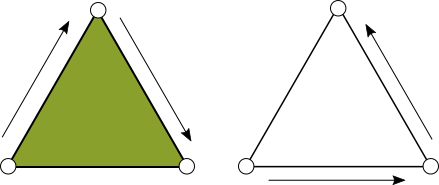
\includegraphics[width=0.6\textwidth]{img/21-1}
	\caption{Ilustracija redoslijeda točaka u smjeru kazaljke na satu i u smjeru obrnutom od kazaljke na satu}
	\label{fig:21-1}
\end{figure}

\paragraph{}
Za generiranje modela u 3D prostoru koji će se uspješno rasterizirati potrebno je osigurati 
da su točke koje tvore lica poredane u smjeru kazaljke na satu zbog optimizacija prilikom
rasteriziranja. Slika \ref{fig:21-1} prikazuje moguće redoslijede definiranja točaka koje 
tvore lice s točkom u donjem lijevom kutu kao početnom točkom za definiranje lica. Zelena boja označava lice koje će se rasterizirati iz trenutnog kuta gledišta.

\begin{figure}[h]
	\centering
	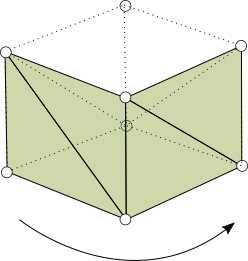
\includegraphics[width=0.45\textwidth]{img/21-2}
	\caption{Šetnja oko modela za popunjavanje lica}
	\label{fig:21-2}
\end{figure}

\paragraph{}
Uzimajući u obzir redoslijed točaka unutar lica, potrebno je generirati sva lica 3D modela 
kako bi svako lice bilo vidljivo iz kuta gledišta u kojem treba biti vidljivo. Jednostavan 
način za vizualizaciju tog postupka prikazan je na slici \ref{fig:21-2}. Krenuvši od 
početne točke generiramo samo ona lica koja bi bila vidljiva iz neke točke gledišta. 
Rotiramo točku gledišta oko modela i dodajemo lica koja su vidljiva iz točke gledišta, a 
nisu prije bila dodana. Nakon vraćanja u početni položaj, sva lica vidljiva iz kuta 
gledišta su popunjena. Proces je potrebno ponoviti na različitim visinama točke gledišta 
kako bi se popunila i lica koja omeđuju model s gornje i donje strane.


\section{Generiranje točaka i lica modela biljaka}
\paragraph{}
Generiranje točaka biljaka vrši se ekstrapolacijom osnovnog oblika biljke na različite 
visine. Osnovni oblik biljke je presjek biljke sa horizontalnom ravninom. Za primjer 
trstike osnovni oblik je krug, a trave paralelogram. Slika \ref{fig:22-1} prikazuje 
vizualizaciju dobivanja osnovnog oblika biljke za tulipan i travku.

\begin{figure}[h]
	\centering
	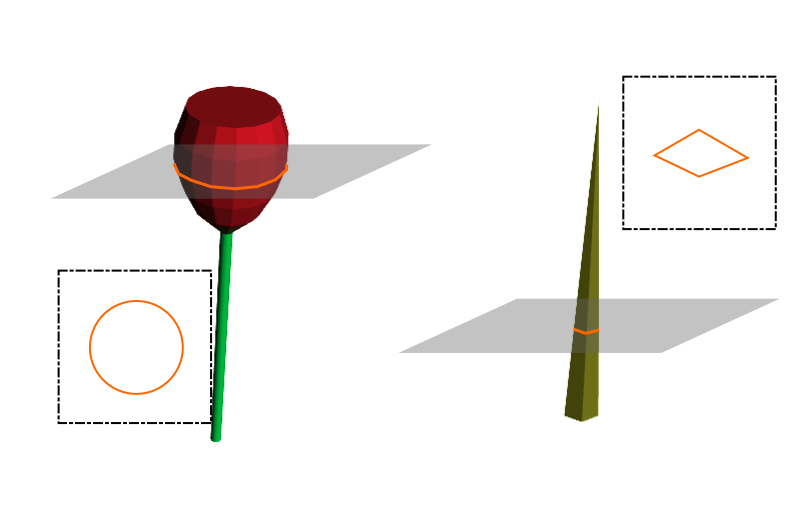
\includegraphics[width=0.8\textwidth]{img/22-1}
	\caption{Dobivanje osnovnog oblika biljke}
	\label{fig:22-1}
\end{figure}

\paragraph{}
Nakon postavljanja početnog oblika, točke osnovnog oblika se postavljaju kao korijen biljke 
i dodaje se novi prsten osnovnog oblika na fiksnim intervalima visine. Svaki prsten ima 
svoju određenu širinu oko centralne točke koja se dobiva iz opisne funkcije biljke. Konstruiranje opisne funkcije biljke opisano je u \ref{usage_tutorial}. Slika \ref{fig:22-2} prikazuje ekstrapolaciju točaka trave, kojima je osnovni oblik paralelogram.

\begin{figure}[h]
	\centering
	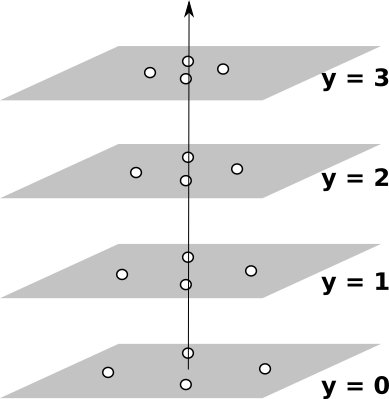
\includegraphics[width=0.45\textwidth]{img/22-2}
	\caption{Ekstrapolacija točaka trave}
	\label{fig:22-2}
\end{figure}

\paragraph{}
Generirane točke spajaju se u model dodavanjem lica. Dodavanje lica se vrši šetnjom gledišta oko generiranih točaka. Postupak dodavanja lica na generirane točke opisan je u poglavlju \ref{generation_basics}. Slika \ref{fig:22-3} prikazuje postupak omatanja u dvije različite iteracije. Tamnije obojana lica reprezentiraju lica koja gledaju u smjeru suprotnom od trenutnog gledišta.

\begin{figure}[h]
	\centering
	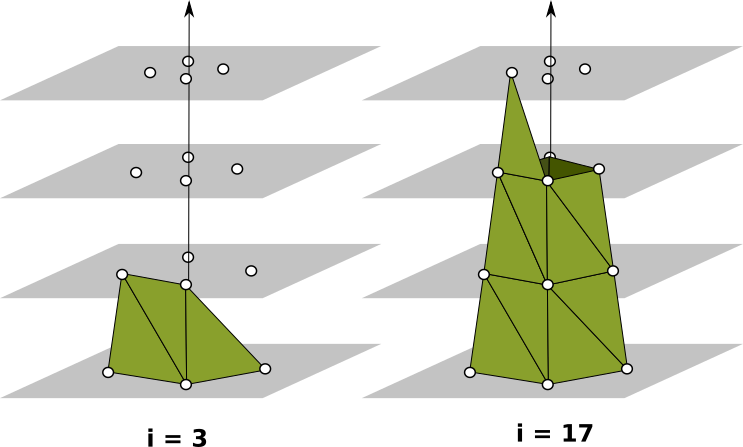
\includegraphics[width=0.75\textwidth]{img/22-3}
	\caption{Spajanje točaka u model kroz iteracije}
	\label{fig:22-3}
\end{figure}

\paragraph{}
Neke osnovne biljke i njihove generacijske funkcije uključene su u prezentirano rješenje i 
mogu se generirati preko korisničkog sučelja. Korisničko sučelje za generiranje modela 
biljaka prikazano je na slici \ref{fig:22-4}.

\begin{figure}[h]
	\centering
	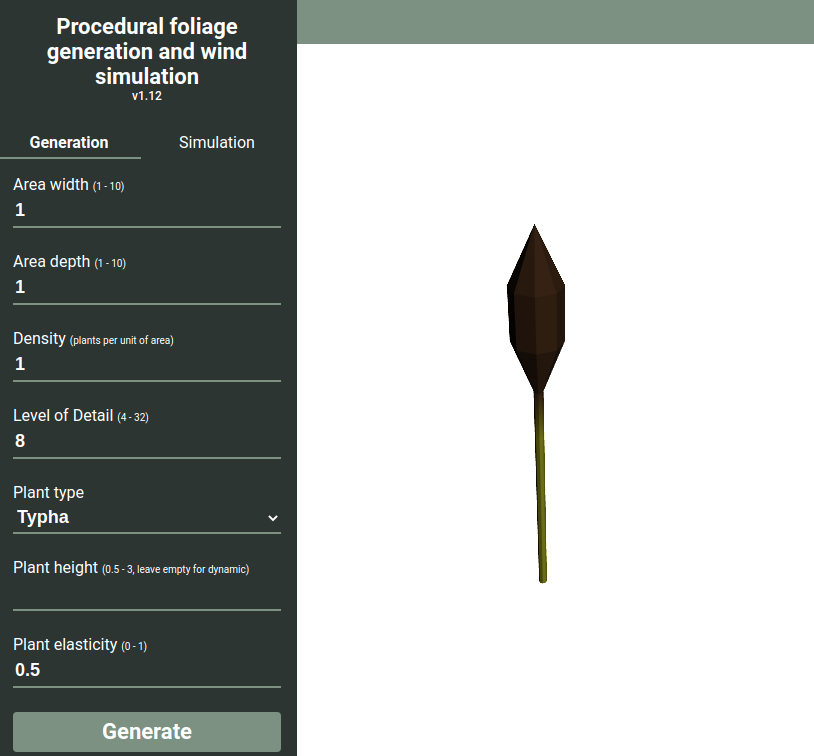
\includegraphics[width=0.75\textwidth]{img/22-4}
	\caption{Korisničko sučelje za generiranje modela biljaka}
	\label{fig:22-4}
\end{figure}

\section{Generiranje modela uz različitu razinu detalja}
\paragraph{}
Različite razina za sve biljke detalja uvjetovane su brojem vertikalnih segmenata na koje je 
biljka razdvojena po svojoj visini. Veći broj segmenata rezultira većom razinom detalja. 
Razdvajanje biljaka po vertikalnim segmentima prikazano je na slici \ref{fig:221-1}. 
Dodavanjem većeg broja segmenata biljka dobiva sve više točaka te na taj način objekt dobiva 
i više detalja. Sijenčanje takvog modela rezultira postepenim prijelazom između boja. Kod 
modela s malim brojem segmenata, promjene u intenzitetu osvjetljenja su mnogo izraženije što 
je također vidljivo na slici \ref{fig:221-1}.

\begin{figure}[h]
	\centering
	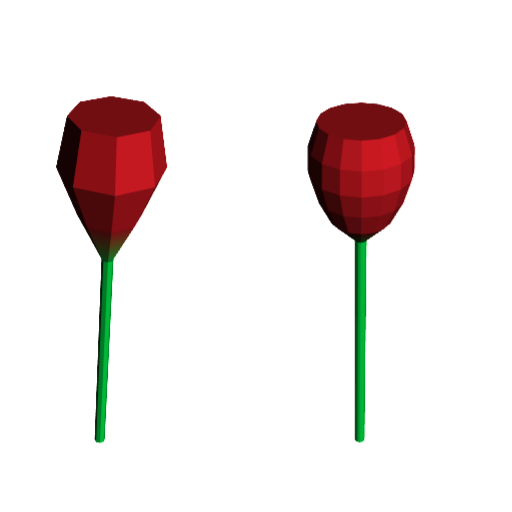
\includegraphics[width=0.45\textwidth]{img/221-1}
	\caption{Generirane biljke sa različitim brojem vertikalnih segmenata}
	\label{fig:221-1}
\end{figure}

\paragraph{}
Osim razine detalja po vertikalnim segmentima, moguće je osnovni oblik biljke uvjetovati po 
količini detalja te time dobiti dodatne karakteristike kod prikaza s više detalja. Primjer 
generiranja osnovnog oblika u većoj ili manjoj razini detalja za osnovni oblik kruga 
ilustrirano je slikom \ref{fig:221-2}, a implementacija tog primjera prikazana je isječkom 
\ref{code25-2}.

\begin{figure}[h]
	\centering
	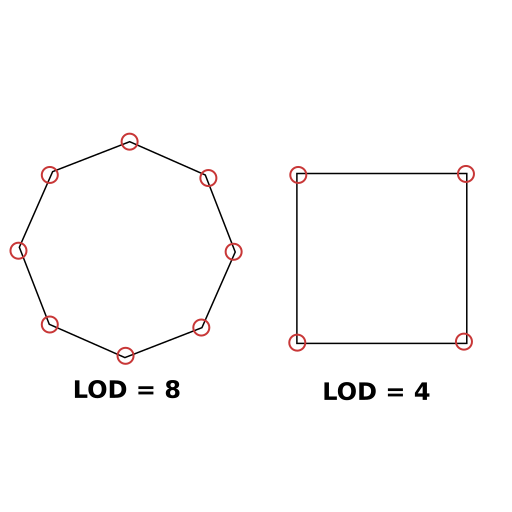
\includegraphics[width=0.45\textwidth]{img/221-2}
	\caption{Prikaz ovisnosti baze kruga o razini detalja prikaza}
	\label{fig:221-2}
\end{figure}

\section{Programska implementacija generiranja i prikaza}
\paragraph{}


\section{Primjer korištenja razvijenog programa za generiranje jednostavne proizvoljne biljke} \label{usage_tutorial}
\paragraph{}
Generiranje biljke prezentiranim rješenjem je jednostavno. Potrebno je definirati svega 
nekoliko svojstava. Oblik baze, visinu biljke, širinu na pojedinim dijelovima te opcijanalno 
boju na dijelovima biljke. Slika \ref{fig:25-1} prikazuje završeni model tulipana 
objašnjenog u ovom primjeru.

\begin{figure}[h]
	\centering
	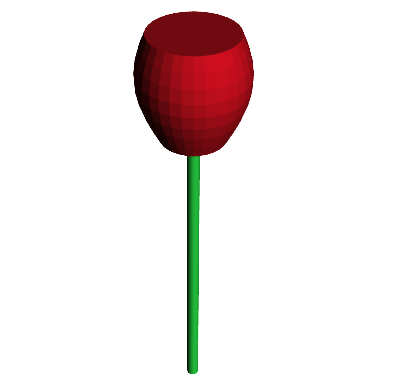
\includegraphics[width=0.6\textwidth]{img/25-1}
	\caption{Prikaz završenog modela tulipana}
	\label{fig:25-1}
\end{figure}

\paragraph{}
Prije opisa biljke potrebno je osigurati apstraktna svojstva biljke naslijeđivanjem razreda
$BaseGenerationFunction$. Postupak je vidljiv u isječku koda \ref{code25-1}.

\begin{lstlisting}[language=Javascript,caption=Naslijeđivanje razreda BaseGenerationFunction,label=code25-1]
import {BaseGenerationFunction} from "base-generation-function.js";
export class TulipFunction extends BaseGenerationFunction {
}
\end{lstlisting}

\paragraph{}
Nakon naslijeđivanja, potrebno je generirati osnovni oblik biljke. Osnovni oblik biljke 
možemo zamisliti kao presjek biljke i horizontalne ravnine. U slučaju tulipana to je krug.
Skup točaka koje reprezentiraju krug možemo izračunati kretanjem po jediničnoj kružnici, i 
na svakom pomaku trigonometrijskim funkcijama $sin$ i $cos$ izračunati koordinate na 
trenutnom koraku. Koordinatu y fiksiramo na 0 za dobivanje točaka u istoj horizontalnoj 
ravnini. Isječak koda \ref{code25-2} prikazuje taj postupak. Opis baznog oblika vrši se u 
metodi $getBaseShape$. Metoda $getBaseShape$ prima parametar $lod$ koji opisuje u kojoj 
razini detalja generiramo biljku.

\paragraph{}
\begin{lstlisting}[language=Javascript,caption=Generiranje osnovnog oblika biljke,label=code25-2]
getBaseShape(lod) {
		if (!lod || lod < 4) {
		lod = 4;
	}

	const vertices = [];
	let i = 0;
	while (i < lod) {
		const offset = i / lod;
		vertices.push([
			-Math.cos(offset * Math.PI * 2) * 0.3,
			0,
			Math.sin(offset * Math.PI * 2) * 0.3
		]);

		i++;
	}

	return vertices;
}
\end{lstlisting}

\paragraph{}
Nakon generiranja osnovnog oblika, potrebno je definirati pretpostavljenu visinu biljke.
U ovom primjeru je ta visina nasumična između 1.2 i 2.2 jedinica u trodimenzijskom 
prostoru. Isječak koda \ref{code25-3} prikazuje definiranje pretpostavljene visine biljke.
\paragraph{}
\begin{lstlisting}[language=Javascript,caption=Generiranje visine biljke,label=code25-3]
generateHeight() {
	return Math.random() + 1.2;
}
\end{lstlisting}
\paragraph{}
Slika \ref{fig:25-2} pokazuje rezultat generiranja sa definiranim osnovnim oblikom i 
pretpostavljenom visinom.

\begin{figure}[h]
	\centering
	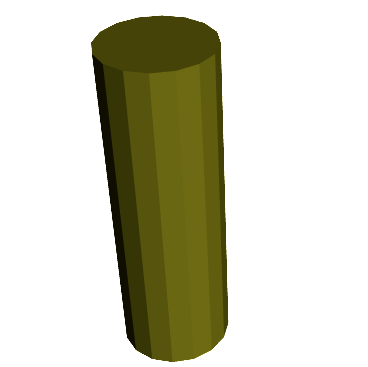
\includegraphics[width=0.6\textwidth]{img/25-2}
	\caption{Rezultat generiranja osnovnog oblika i pretpostavljene visine}
	\label{fig:25-2}
\end{figure}

\paragraph{}
Nakon opisa osnovna dva svojsta, potrebno je definirati zakrivljenost modela. Zakrivljenost 
modela se postavlja u metodi $calculateCurvePoint$. Metoda $calculateCurvePoint$ prima 
parametar $offset$ koji nam govori za koju visinu biljke tražimo širinu. Parametar $offset$ 
je vrijednost između 0 i 1, gdje 0 simbolizira dno biljke, a 1 simbolizira vrh biljke.
Tulipan je biljka tanke stabljike i zvonolikog cvijeta. Za tanku stabljiku vraćamo 
vrijednost širine 0.1, a zvono modeliramo sa pola periode spljoštene sinusoide i bazne 
širine na koju dodajemo amplitudu takve sinusoide. Isječak koda \ref{code25-3} pokazuje opis 
biljke tulipana, a slika \ref{fig:25-3} rezultat pokretanja nakon opisa oblika.
\paragraph{}
\begin{lstlisting}[language=Javascript,caption=Postavljanje oblika biljke u ovisnosti o visinu od tla,label=code25-3]
calculateCurvePoint(offset) {
	if (offset < 0.75) {
		return 0.1;
	}

	const flowerOffset = (offset - 0.75) / 0.3 * Math.PI;
	return 0.5 + Math.sin(flowerOffset) / 3;
}
\end{lstlisting}

\begin{figure}[h]
	\centering
	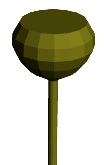
\includegraphics[width=0.2\textwidth]{img/25-3}
	\caption{Rezultat generiranja sa definiranim oblikom biljke}
	\label{fig:25-3}
\end{figure}
\paragraph{}
Dodavanje boje se odvija na sličan način kao definiranje oblika. Dodavanje boje definira se 
u metodi $calculateColorAtPoint$ koja također prima parametar $offset$. Tulipan ima zelenu 
stabiljku i cvijet neke boje. U primjeru je korištena crvena boja cvijeta. Isječak koda 
\ref{code25-4} prikazuje postavljanje boje, a rezultat generiranja i prikazan je na slici 
\ref{fig:21-1}.

\begin{lstlisting}[language=Javascript,caption=Dodavanje boja modelu,label=code25-4]
calculateColorAtPoint(offset) {
	if (offset < 0.75) {
		return [0.2, 0.85, 0.2, 1];
	}

	return [0.8, 0.1, 0.1, 1];
}
\end{lstlisting}


\chapter{Simulacijski model}
\section{Fizički model ponašanja biljke}
\paragraph{}
Osnovne sile koje utječu na ponašanje biljke su sila teža, unutrašnji otpor 
biljke i vanjski utjecaji. Sila teža konstantnim intenzitetom gura sve dijelove 
biljke prema dolje. Vanjski utjecaji poput vjetra, djeluju u svim smjerovima 
različitim intenzitetima na različite dijelove biljke. Te unutrašnji otpor 
biljke, koji uvijek djeluje u suprotnom smjeru od preostale dvije sile. Na 
slici \ref{fig:31-1} su slikovito prikazane sile koje djeluju na svaki mikroskopski malen 
dio biljke. Važno je napomenuti da su za tenziju i kompresiju prikazane sile koje one 
uzrokuju, a ne smjer kompresije odnosno tenzije.

\begin{figure}[h]
	\centering
	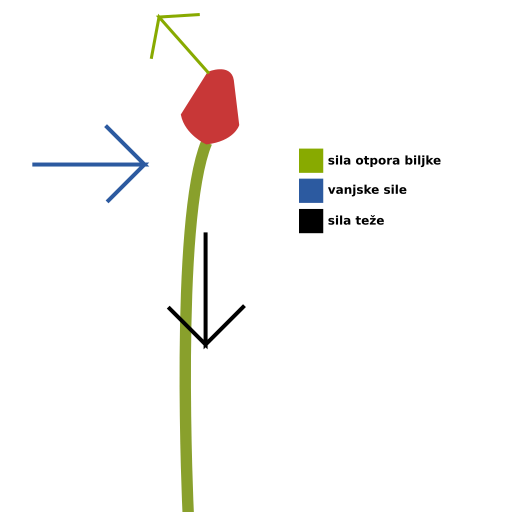
\includegraphics[width=0.75\textwidth]{img/31-1}
	\caption{Prikaz sila koje djeluju na biljku}
	\label{fig:31-1}
\end{figure}

\paragraph{}
Usred djelovanja te tri sile, biljka u svakom trenutku pokušava doći u stanje gdje se te tri 
sile poništavaju. Svako gibanje biljke prouzrokovano je promjenom vanjskih utjecaja kojima 
se biljka pokuša prilagoditi kako bi ukupna sila koja djeluje na biljku bila nula.

\paragraph{}
Čak i naizgled jednostavan problem kao što je simuliranje ponašanja biljke je u svojoj 
naravi izrazito kompleksan. Sila teža djeluje na svaki mikroskopski dio biljke. Na isti 
način djeluju i vanjske sile. Vanjske sile i sila teže u biljci uzrokuju napetosti i 
kompresije koje uzrokuju silu otpora biljke. To sve se događa na mikroskopskoj razini na 
svakom dijelu površine biljke. Savršena simulacija ovakvog sustava bila bi izrazito  
računalno zahtjevna.

\section{Programski model fizičkog ponašanja} \label{physics_model}
\paragraph{}
Zbog računalne zahtjevnosti i problema preciznog definiranja svih sila, potrebno je pronaći
matematički model koji bi rezultirao istim (ili barem vrlo sličnim) ponašanjem, a imao bi 
mnogo manju računalnu složenost i bio bi jednostavniji za definirati.

\paragraph{}
U računalnom programiranju se fizičke interakcije obično modeliraju preko tri osnovna  
građevna bloka. Tijela, ograničenja i sile. Tijela su geometrijski oblici u tro-
dimenzijskom prostoru koja zauzimaju volumen i podložna su djelovanju sila. Ograničenja 
su skup pravila koja određuju kako se neka dva tijela mogu ponašati relativno jedno prema 
drugom. Sile djeluju na tijela i uzrokuju promjene koje se tada na temelju ograničenja 
rješavaju.

\paragraph{}
Primjer tijela je kocka u trodimenzijskom prostoru. Primjer sile je sila teža koja djeluje 
konstantnim intenzitetom prema negativnoj y osi. Primjer ograničenja je ako se volumen 
jednog tijela nađe unutar volumena drugog tijela, na oba tijela se primjenjuje sila u smjeru 
suprotnom od središta mase drugog tijela. Ovo ograničenje je naivni pristup rješavanju 
kolizija između tijela.

\paragraph{}
Stvarnu simulaciju jednostavne biljke možemo vrlo dobro aproksimirati korištenjem svega dva 
tijela, jednog ograničenja i jedne sile koja djeluje na jedno od tijela. Ovaj jednostavni model prikazan je slikom \ref{fig:32-1}.

\begin{figure}[h]
	\centering
	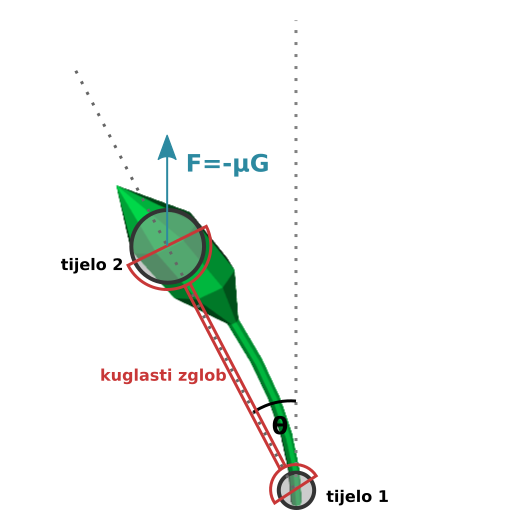
\includegraphics[width=0.8\textwidth]{img/32-1}
	\caption{Ilustracija prikaza fizičkog modela stvarnog gibanja}
	\label{fig:32-1}
\end{figure}

\paragraph{}
Tijelo 1 u fizičkom modelu predstavlja korijen biljke i u simulaciji je u cijelosti 
statično. Tijelo 2 predstavlja vrh biljke i dinamičko je, odnosno može reagirati na utjecaj
sila. Ta dva tijela spojena su kuglastim zglobom. Kuglasti zglob je ograničenje na tijelo 2 
koje dozvoljava tijelu da se slobodno giba i rotira u prostoru oko bilo koje osi pod uvjetom 
da je uvijek jednako udaljeno od tijela 1.

\paragraph{}
Na tijelo 2 također djeluje sila F koja je svojim smjerom obrnuta od smjera sile teže, a 
njezin iznos je određen kutom otklona od neutralne pozicije. Neutralna pozicija ima tijelo 2 
direktno iznad tijela 1 i u takvom slučaju je faktor $\mu$ jednak 0.

\paragraph{}
Računanje otklona $\theta$ u trodimenzijskom prostoru radimo kao omjer duljine 
stranica trokuta. Jedna od stranica je projekcija pozicije tijela 2 na ravninu 
xz, a druga stranica je visina tijela 2 iznad te ravnine. Zbog kuglastog zgloba 
očekujemo da je duljina vektora pozicije tijela 2 od ishodišta uvijek jednaka, 
normalizacijom pozicije tijela 2, duljina projekcije na xz ravninu ima 
vrijednost $cos$ kuta $\theta'$. Zanimljiva informacija nam je otklon od y osi, koristimo 
$sin(\theta')$ te vrijednost kako bi dobili suprotan kut ($\pi / 2 - \theta'$). U takvom 
slučaju nam je dovoljna informacija uzeti y vrijednost normalizirane pozicije i možemo 
precizno izračunati otklon. Računanje kuta otklona prikazano je formulom \ref{eq:32-1}.

\begin{equation}
\theta = asin(normalized(position).y)
\label{eq:32-1}
\end{equation}

\begin{figure}[h]
	\centering
	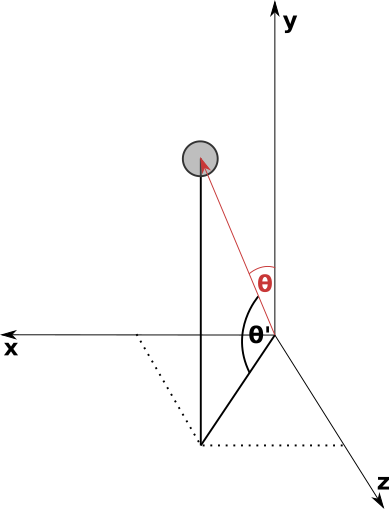
\includegraphics[width=0.5\textwidth]{img/32-2}
	\caption{Prikaz izračuna kuta otklona}
	\label{fig:32-2}
\end{figure}


\paragraph{}
Nakon izračuna kuta otklona, računanje sile koja djeluje na tijelo 2 je sada jednostavno i 
prikazano formulom \ref{eq:32-2}. Računanje sile je također proporcionalno sa sinusom kuta 
na intervalu između 0 i 90 stupnjeva. Sila koja djeluje na tijelo kod otklona većeg od 90 
stupnjeva veća je od sile koja djeluje na tijelo na otklonu manjem od 90 stupnjeva. Kod 
jednostavnog modela s jednim zglobom ovo je nerealan slučaj jer se tijelo 2 ne može naći u  
takvoj poziciji (tijelo 2 bi tada bilo ispod tijela 1, i prošlo bi kroz površinu poda), ali 
ga je bitno spomenuti zbog skaliranja na model s većim brojem zglobova.

\begin{equation}
\vec{F} = sin(\theta) \cdot (1 + elasticity) \cdot \vec{G} \cdot (-1)
\label{eq:32-2}
\end{equation}

\paragraph{}
Rezultirajuća sila $\vec{F}$ djeluje u negativnom y smjeru (suprotno od smjera sile teže).
Takav smjer je rezultat faktora $\vec{G} \cdot (-1)$. U formuli se javlja i faktor $(1 + 
elasticity)$. Njegova zadaća je osigurati da biljke koje imaju veći faktor elastičnosti 
stoje bliže centru ravnoteže čak i kod malih otklona od središta. Primjer biljke koja ima 
velik faktor elastičnosti je rogoz, koji stoji potpuno uspravno u neutralnoj poziciji. 
Primjer male elastičnosti biljke je zvončić, koji nema dovoljno sile kako bi se vratio u 
neutralni (uspravni) položaj. Ime faktora je elastičnost jer odgovara na pitanje kolikom 
silom će se biljka pokušati vratiti u neutralni položaj nakon što je otklonjena od centra 
ravnoteže.

\subsection{Usporedba sila programskog i fizičkog modela}
\paragraph{}
Zbrajanjem svih komponenata sila po cijeloj površini biljke dobivamo jednu 
reprezentativnu silu koja dijeluje na biljku. Tu reprezentativnu silu možemo razdvojiti na 
tri komponente - horizontalnu, vertikalnu i silu na tangenti kružnice oko centra rotacije. 
Horizontalna sila je razlika između sile vjetra i horizontalne komponente unutrašnje sile 
otpora biljke koja se opire toj sili vjetra. Vertikalna sila je razlika između sile teže 
koja djeluje na biljku i vertikalne komponente unutarnje sile otpora biljke koja se odupire 
sili teži. Treća komponenta sile je sila tangencijalna na centar rotacije biljke. 
Tangencijalna sila je prividna sila koja pokušava vratiti biljku u početni položaj. Na slici 
\ref{fig:321-1} prikazane su sume sila koje djeluju na biljku.

\begin{figure}[h]
	\centering
	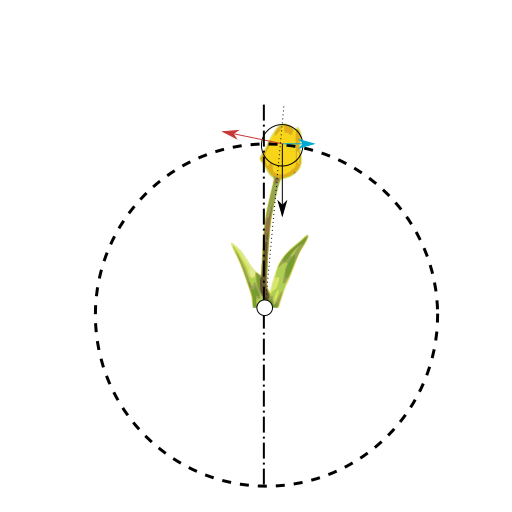
\includegraphics[width=0.7\textwidth]{img/321-1}
	\caption{Komponente rezultatne sile koje djeluju na gornji dio biljke}
	\label{fig:321-1}
\end{figure}

\paragraph{}
U programskom modelu fizičkog ponašanja biljke imamo samo jednu aktivnu silu koja je 
zadužena za simuliranje ponašanja unatrašnjeg otpora. Iako ta sila ima isključivo vertikalni 
smjer, fizički model i dalje pokazuje horizontalno ponašanje. Razlog ponašanja koje prati 
fizičko ponašanje čak i slučaju kada ne simuliramo sve sile je ograničenje kuglastog zgloba.
Kuglasti zglob implicitno primjenjuje silu preko svojih pravila. Primjenom sile prema gore, 
tijelo koje reprezentira vrh biljke pokušava se gibati prema gore, gibanjem prema gore 
udaljava se od tijela korijena biljke. Kuglasti zglob osigurava jednako udaljenost između 
tijela pomicanjem tijela vrha biljke u horizontalnom smjeru.

\paragraph{}
Fizički pokretač ne djeluje silom da bi pomaknuo tijelo u horizontalnom smjeru, već mijenja 
poziciju direktno. Ali čak i takvo rješenje daje uvjeriljivu simulaciju.


\section{Programska implementacija fizičkog modela}
\paragraph{}
Fizički pokretač korišten u prezentiranom rješenju je OimoPhysics. Taj pokretač je napisan
u programskom jeziku Haxe i preveden u programski jezik Javascript. Izbor ovog fizičkog 
pokretača prvenstveno je potaknut njegovom relativnom jednostavnošću i njegovom mogućnosti 
izvršavanja direktnog izvođenja unutar preglednika. Zbog jednostavnog modela kojeg 
simuliramo, nije predana velika težina performansama koje zbog izvođenja u interpretiranom
jeziku mogu negativno utjecati na brzinu izvođenja programskog rješenja.

\paragraph{}
Osnova svakog fizičkog pokretača je svijet simulacije (engl. \textit{world}) koji sadržava 
sve osnovne gradivne blokove fizičke simulacije objašnjene u sekciji \ref{physics_model}.
Svijet implicitno definira ograničenja za rješavanje kolizija između objekata. Inicijalno
postavljanje vrijednosti svijeta u OimoPhysics pokretaču je iznimno jednostavno i prikazano je isječkom koda \ref{code33-1}.
\paragraph{}

\begin{lstlisting}[language=Javascript,caption=Postavljanje simulacijskog svijeta, label=code33-1]
const world = new OIMO.World(1, new Vec3(0, -9.81, 0))
\end{lstlisting}

\paragraph{}
Prvi parametar kod inicijalizacije je izbor algoritma rješavača kolizija (engl. \
\textit{collision-solver}. Različiti algoritmi pridaju različite važnosti pojedinim 
elementima simulacije. Za znanstvene radove izabrali bi algoritam koji manju pažnju pridaje
brzini izvođenja simulacije, a veću pažnju točnosti same simulacije. Za igre i ostale 
sustave koji se izvršavaju u stvarnom vremenu, manje nam je bitna točnost, a bitnija je 
brzina izvođenja. Algoritmi unutar OimoPhysics pokretača su označeni od 0 do 2, gdje 
vrijednost implicira kolika se težina pridaje točnosti simulacije. U prezentiranom radu
korištena je postavka 1, koja postiže balansirani odnos između točnosti i brzine izvođenja.

\paragraph{}
Nakon kreiranja simulacijskog svijeta dodajemo fizički kostur svakoj biljci. Fizički kostur 
biljke sastoji se od 3 dijela. tijela 1 koje je nepomično i opisuje korijen biljke, tijela 2 
koje je vrh biljke i podložno je utjecaju sila te kuglastog zgloba koji povezuje tijelo 1 i
tijelo 2.

\paragraph{}
Tijelo u simulacijskom svijetu opisano je s dva konfiguracijska objekta. Svaki 
konfiguracijski objekt objašnjava zaseban dio simulacije. Prvi konfiguracijski objekt su
općenita svojstva tijela poput njegove inicijalne pozicije u simulacijskom svijetu i vrsta
ponašanja tijela. Konfiguracijski razred za općenita svojstva tijela u OimoPhysics pokretaču 
je \verb#RigidBodyConfig#. U korištenom fizičkom pokretaču postoje tri vrste
ponašanja tijela - statično, dinamički i kinematičko. Na statična tijela ne utječe sila i 
ne mijenjaju svoju poziciju i rotaciju čak ni prilikom kolizije s drugim tijelima. Na 
dinamička tijela utječe sila i ona se ponašaju kao svi objekti u stvarnom svijetu - prilikom 
kolizije se odbijaju i rotiraju, a prilikom djelovanja sile ubrzavaju ili usporavaju u 
smjeru sile. Dinamička tijela reagiraju na koliziju sa statičnim i kinematičkim tijelima. 
Kinematička tijela ne reagiraju na kolizije, ali reagiraju na sile i njihovim utjecajem mogu 
mijenjati svoju poziciju i rotaciju.
\paragraph{}

\begin{lstlisting}[language=Javascript, caption=Postavljanje tijela korijena biljke i njegovih svojstava,label=code33-2]
const origin = new OIMO.Vec3(
	plant.pos[0], plant.pos[1], plant.pos[2]
);

const baseConfig = new OIMO.RigidBodyConfig();
baseConfig.position = origin;
baseConfig.type = OIMO.RigidBodyType.STATIC;

let shapeConfig = new OIMO.ShapeConfig();
shapeConfig.geometry = new OIMO.BoxGeometry(
	new OIMO.Vec3(0.1, 0.1, 0.1)
);

const base = new OIMO.RigidBody(baseConfig);
base.addShape(new OIMO.Shape(shapeConfig));

this.world.addRigidBody(base);
\end{lstlisting}

\paragraph{}
Za tijelo koje simulira korijen biljke pozicija tijela odgovara poziciji tijela u 3D 
prikazu. Vrsta tog tijela je statična. Ne mijenja svoju poziciju i na rotira se. Ovakvo
ponašanje prati ponašanje stvarnih biljaka u normalnim atmosferskim uvjetima.

\paragraph{}
Drugi konfiguracijski razred je \verb#ShapeConfig#. \verb#ShapeConfig# opusuje geometriju 
modela u 3D prostoru. U fizičkim pokretačima uobičajeno je pojednostaviti geometriju modela
što je više moguće kako bi brzina izvođenja bila što veća. Iz tog razloga su geometrije 
tijela obično jednostavni geometrijski oblici poput kvadra, kugle, piramide i stošca.
Složeniji oblici mogu se dobiti dodavanjem dodatnih jednostavnih oblika na tijelo.

\paragraph{}
Tijelo koje simulira korijen biljke je statično i nema interakciju s ostalim tijelima, pa je
u prezentiranom rješenju opisan samo kao mala kocka na dnu biljke. Postavljanje svojstava 
tijela korijena biljke i njegove geometrije prikazano je u isječku koda \ref{code33-2}.

\paragraph{}
Tijelo koje simulira vrh biljke iako složenije, također ima vrlo jednostavan proces 
postavljanja početnih vrijednosti. Pozicija tijela je točno iznad tijela korijena biljke na
y vrijednosti koja odgovara visini biljke. Vrsta ovog tijela je dinamičko, jer osim 
reagiranja na sile vjetra reagira i kod potencijalnih interakcija s ostalim biljkama. 
Promjene koje sadrži postavljanje početnih vrijednosti tijela vrha biljke u odnosu na tijelo 
korijena prikazan je isječkom koda \ref{code33-3}.

\begin{lstlisting}[language=Javascript,label=code33-3,caption=Postavljanje tijela vrha biljke]
...
tipConfig.position = origin.add(new OIMO.Vec3(0, plant.height, 0));
tipConfig.type = OIMO.RigidBodyType.DYNAMIC;

...
shapeConfig.geometry = new OIMO.SphereGeometry(
	plant.collisionRadius
);
\end{lstlisting}

\paragraph{}
Vrh biljke umjesto kocke ima kuglu. Iako neprecizno, kugla dobro opisuje ponašanje 	
interakcije vrha biljaka i pogodno je za brzinu izvođenja.

\paragraph{}
Definicija kuglastog zgloba u OimoPhysics pokretaču također je jednostavna. Sastoji se od
jednog konfiguracijskog objekta koji opisuje sva svojstva ovog ograničenja.
Taj konfiguracijski razred je \verb#SphericalJointConfig#. \verb#init# metodi ovog 
konfiguracijskog objekta predajemo tijela na koja će se ovo ograničenje primjenjivati. U 
prezentiranom rješenju to su tijela \verb#base# i \verb#tip#. Osim tijela na koja se 
ograničenje primjenjuje potrebno je definirati i referentnu točku za to ograničenje. Kod 
simulacije se vrh biljke rotira oko korijena biljke, pa poziciju korijena biljke uzimamo kao 
referentnu točku.
\paragraph{}

\begin{lstlisting}[language=Javascript,label=code33-4,caption=Postavljanje kuglastog zgloba]
const jointConfig = new OIMO.SphericalJointConfig();
jointConfig.init(base, tip, baseConfig.position);
jointConfig.springDamper = new OIMO.SpringDamper().setSpring(0, 0);
jointConfig.breakForce = 0;
jointConfig.breakTorque = 0;

const joint = new OIMO.SphericalJoint(jointConfig);
this.world.addJoint(joint);
\end{lstlisting}

\paragraph{}
U ostatku konfiguracije definiran je i prigušivač opruge. Prigušivač opruge simulira 
ograničenje kao oprugu umjesto čvrstu vezu između tijela. U prezentiranom rješenju postavke
prigušivača su postavljene na nulu. Ovakve postavke postavljaju ograničenje kao čvrstu vezu
između dva tijela. Biljke možemo zamisliti kao opruge pa ovakav izbor djeluje nelogično. 
Odabir baš takvih parametara rezultat je ručne implementacije vrlo sličnog ponašanja biljke.
Korištenje oba sustava za simulaciju elastičnosti rezultira fizičkim nekonzistencijama u 
ponašanju biljke.

\paragraph{}
Parametri \verb#breakForce# i \verb#breakTorque# opisuju silu i obrtni moment pod kojim bi
ograničenje popustilo, odnosno prestalo raditi. Vrijednost nula u konfiguraciji signalizira
fizičkom pokretaču da je ograničenje konstantno, odnosno da neće prestati vrijediti bez 
obzira na sile koje djeluju na tijela. Cijelovito postavljanje vrijednosti ograničenja 
kuglastog zgloba prikazano je isječkom koda \ref{code33-4}.

\paragraph{}
Nakon početnog postavljanja kostura biljke potrebno je definirati ponašanje biljke u 
simulaciji. Definicija ponašanja prikazana je u isječku koda \ref{code33-5}. U simulaciji
prolazimo kroz sve kuglaste zglobove u kosturu biljke i izvršavamo simulaciju za svaki od 
njih. U jednostavnim primjerima postoji samo jedan zglob za svaku od biljaka, ali na ovaj 
način je sačuvana mogućnost simuliranja mnogo složenijih konfiguracija.

\paragraph{}
Na početku jedne iteracije simulacije uzimamo tijela na koja je primijenjeno ograničenje
kuglastog zgloba. Na drugo tijelo (vrh biljke) primjenjujemo silu vjetra. Sila vjetra 
je vektor neke duljine u 3D prostoru. Duljina vektora odgovara snazi koju vjetar ima u nekom 
trenutku. Nakon primjene sile vjetra, na tijelo se primjenjuje izrazito mala sila koja 
djeluje suprotno od vektora brzine tijela. Tijelo zbog te sile konstantno usporava i 
time rješava problem beskonačne simulacije čak i za vrlo male i kratkotrajne početne sile.

\paragraph{}
\begin{lstlisting}[language=Javascript,label=code33-5,caption=Fizička simulacija ponašanja biljke.]
simulateMovement() {
	for (const joint of this.skeleton.joints) {
		const rigid1 = joint.getRigidBody1();
		const rigid2 = joint.getRigidBody2();

		this.applyWind(rigid2);
		this.applyInnerFriction(rigid2);

		// we need relative position of joint
		const pos1 = rigid1.getPosition();
		const pos2 = pos1.sub(rigid2.getPosition());

		const force = Math.abs(this.forceFactor(pos2));
		rigid2.applyForceToCenter(new OIMO.Vec3(0, force, 0));
	}
}
\end{lstlisting}

\paragraph{}
Nakon završene simulacije vjetra računamo silu koja objašnjava ponašanje biljke na 
vjetru. Sila je detaljno objašnjena u poglavlju \ref{physics_model}. Funkcija 
\verb#forceFactor# računa iznos sile kojom djelujemo, a opisana je formulama \ref{eq:32-1} i 
\ref{eq:32-2}.

\chapter{Simulacija ponašanja generiranog modela}
\section{Povezivanje fizičkog modela i modela prikaza}
\paragraph{}
Do sada su definirana dva odvojena sustava, sustav fizičke simulacije i sustav prikaza. 
Fizički sustav je definiran preko dva tijela i jednog zgloba koji imaju odnose roditelj-
dijete. Tijelo koje ima ulogu korijena biljke je roditelj, tijelo koje simulira vrh biljke 
je dijete tog tijela, a ograničenje koje ih povezuje je veza između njih. U računalnoj 
grafici postoji sličan koncept zapisa poze nekog složenog sustava. Takav način 
hijerarhijskog zapisa naziva kostur (engl. \textit{skeleton}), u kojem su pohranjeni podaci 
o djeci - kostima (engl. \textit{bones}).

\paragraph{}
Fizički sustav opisan u cjelini 3 možemo opisati kosturom od dvije kosti. Prva kost 
nema roditelja, pozicionirana je na referentnoj točki fizičkog sustava i ima 
konstantnu rotaciju koja uvijek gleda prema pozitivnoj y osi (prema gore). Druga kost 
je dijete prve kosti i rotirana je tako da uvijek gleda u smjeru vektora između tijela 1 
i tijela 2.

\paragraph{}
Nakon definiranja kostura, potrebno je definirati način na koji će se grafički model 
mijenjati prema promjenama pozicija i rotacija kostiju. Ovaj postupak se zove omatanje 
(engl. \textit{skinning}). Omatanje se vizualno može objasniti kao dodavanje utjecaja kosti 
na pojedine točke u prostoru, tako da je kost uvijek bude unutar volumena koje te točke 
zatvaraju. Primjer ilustracije omatane mreže točaka prikazan je na slici \ref{fig:41-1}.

\paragraph{}
Svaka kost je definirana preko matrice. U matrici su podaci o poziciji kosti te njenoj 
orijentaciji. Način na koji točka unutar prikaza poprima te karakteristike je jednostavnim 
množenjem pozicije točke s matricom kosti.

\begin{figure}[h]
	\centering
	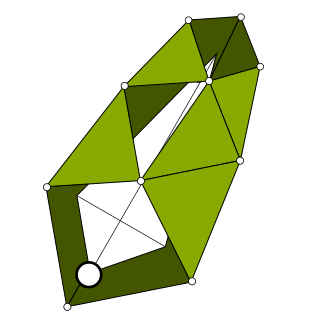
\includegraphics[width=0.7\textwidth]{img/41-1}
	\caption{Ilustracija omotane mreže točaka oko kosti}
	\label{fig:41-1}
\end{figure}

\paragraph{}
Kod savršenog omatanja utjecaj na jednu točki ima samo jedna kost. U praksi, kao i u 
prikazanom rješenju to nije uvijek slučaj. Korištenjem savršenog omatanja dobili bi biljku 
koja se u korijenu uvijek rotira prema smjeru vjetra. Takva biljka bila bi ravna i ne bi 
djelovala prirodno. 

\paragraph{}
Način na koji se rješava taj problem je dodavanjem težina utjecaja kosti na pojedinu točku u 
modelu. Težina je vektor decimalnih brojeva između jedan i nula, gdje jedinica označava 
potpun utjecaj neke kosti na točku, a nula označava da ta kost nema nikakav utjecaj na 
točku.

\paragraph{}
U primjeru simuliranja biljke na vjetru, točke koje su bliže korijenu su pod manjim 
utjecajem kosti koja uzrokuje rotaciju od točaka koje su bliže vrhu. Rezultat takve 
raspodjele težina jasno je vidljiv na slici \ref{fig:32-1}.

\paragraph{}
Zbog jednostavnosti problema, način na koji su težine raspodijeljene je linearan s obzirom 
na visinu biljke. Točke na samom dnu biljke imaju težinu prema rotirajućoj kosti nula, a 
prema statičnoj kosti jedan. Rastom visine, odnosno y vrijednosti pozicije pojedine točke, 
težina kojom statična kost utječe na točku opada, a težina kojom rotirajuća kost utječe 
raste. Izračun težine za pojedinu točku prikazan je formulom \ref{eq:41-1}.

\begin{equation}
w = vertexHeight / plantHeight
\label{eq:41-1}
\end{equation}

\section{Programska implementacija modela}
\paragraph{}
Izračun pozicije točke u prostoru pod utjecajem kosti izvršava se na grafičkoj kartici. Prošireni program sjenčanja s omatanjem prikazan je u isječku \ref{code42-1}.

\paragraph{}
\begin{lstlisting}[language=Javascript,label=code42-1,caption=Proširenja programa za sjenčanje omatanjem]
...
attribute vec4 a_weights;

...
uniform mat4 u_bone;

void main() {
	float counterWeight = 1.0 - a_weights[0];
	gl_Position = u_worldViewProjection * (
		u_bone * a_position * a_weights[0] +
		a_position * counterWeight
	);
	
	...
}
\end{lstlisting}

\paragraph{}
Kost korijena biljke je konstantna pa ju zbog jednostavnosti ne šaljemo prema grafičkoj 
kartici. 

\paragraph{}
\verb#a_weights# je vektor utjecaja kostiju na točku u prostoru. Koristimo samo prvu 
vrijednost iz vektora jer imamo samo jednu kost koja vrši animaciju. Korištenje vektora je 
zadržano zbog potencijalnih nadogradnji u budućnosti. Također, korištenje vektora ne utječe 
na performanse jer se prema grafičkoj kartici šalje samo jedan podatak, a ostala tri su 
pretpostavljene vrijednosti. Ovakav vektor u teoriji podržava 4 različite kosti.

\paragraph{}
\verb#u_bone# je matrica rotirajuće kosti u prikazu. U glavnom dijelu programa izračunava se 
protu-težina. Odnosno, koliko utjecaja na točku u prostoru ima statična kost. Statična kost 
je matrica identiteta i njenim množenjem pozicije točke u prostoru ne dobivamo nikakvu 
razliku pa je to množenje u programu za sjenčanje izostavljeno.

\paragraph{}
Kada bi statična kost mijenjala svoju poziciju ili rotaciju, nju bi također morali poslati 
prema grafičkoj kartici i izračun pozicija točke bi izgledao kao što je prikazano u isječku 
koda \ref{code42-2}.

\paragraph{}
\begin{lstlisting}[language=Javascript,label=code42-2,caption=Prošireno računanje pozicije točke na dvije kosti]
gl_Position = u_worldViewProjection * (
	u_bone_1 * a_position * a_weights[0] +
	u_bone_2 * a_position * a_weights[1]
);
\end{lstlisting}

\paragraph{}
Kako bi grafička kartica ispravno izračunala pozicije točaka, potrebno joj je u svakoj 
iteraciji poslati matricu rotirajuće kosti. Slanje matrice prema grafičkoj kartici prikazano je isječkom koda \ref{code42-3}.

\paragraph{}
\begin{lstlisting}[language=Javascript,label=code42-3,caption=Slanje dodatnih informacija prema grafičkoj kartici]
let boneMatrix = mat4.xRotation(angles[0]);
boneMatrix = mat4.zRotate(boneMatrix, angles[2]);

const uBone = this.gl.getUniformLocation(
	this.program, shaderBinding
);

this.gl.uniformMatrix4fv(
	uBone,
	false,
	boneMatrix
);
\end{lstlisting}
\paragraph{}

\section{Različiti parametri simulacije}
\paragraph{}
Za bolju ocjenu rezultata potrebno je testirati više različitih parametara simulacije i 
usporediti njihov utjecaj na simulaciju s ponašanjem u stvarnom svijetu. U simulaciji možemo 
utjecati na snagu vjetra, smjer vjetra, vrstu puhanja vjetra i za neke vrste puhanja možemo 
mijenjati frekvenciju puhanja. Prikaz sučelja za podešavanje parametara simulacije prikazan 
je na slici \ref{fig:43-4}.

\begin{figure}[h]
	\centering
	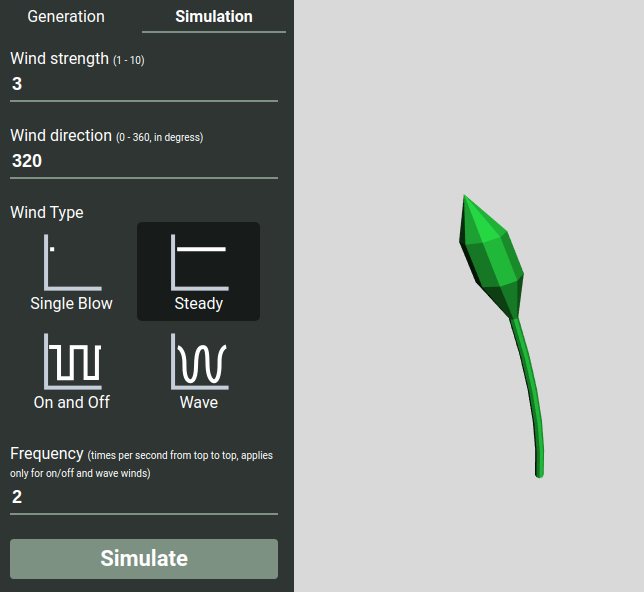
\includegraphics[width=1\textwidth]{img/43-4}
	\caption{Prikaz sučelja za simuliranje vjetra}
	\label{fig:43-4}
\end{figure}

\paragraph{}
Snaga vjetra objašnjava kojim intenzitetom djelujemo na tijelo vrha biljke u jedinici 
vremena. Jedinica vremena u fizičkom pokretaču se naziva korak i traje 32 ms. Snaga vjetra 
10 odgovara sili od 10 N. 

\paragraph{}
Smjer vjetra je predstavljen kutem iz kojeg dolazi u odnosu na biljku. Vjetar pod kutem 0 
stupnjeva djeluje od negativne prema pozitivnoj z osi. Vjetar pod kutem 90 stupnjeva djeluje 
od negativne x osi prema pozitivnoj x osi.

\paragraph{}
U simulaciji postoje 4 vrste vjetra. Udar vjetra puše kratko vrijeme u jednom smjeru i nakon 
toga je njegovo puhanje gotovo. Graf snage puhanja kod udara vjetra prikazan je na slici 
\ref{fig:43-0}.

\begin{figure}[h]
	\centering
	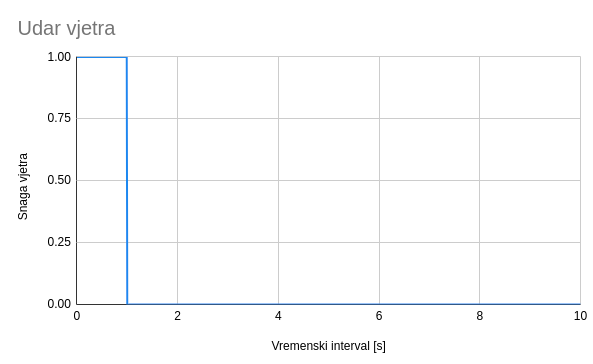
\includegraphics[width=0.8\textwidth]{img/43-0}
	\caption{Funkcija udara vjetra uz parametar snage 1}
	\label{fig:43-0}
\end{figure}

\paragraph{}
Konstantno puhanje djeluje istim inzetitetom u jednom smjeru bez prestanka. Graf konstantnog 
puhanja prikazan je na slici \ref{fig:43-1}. Konstantno puhanje i udar vjetra su jednostavne 
simulacije korištene u razvoju i ne simuliraju dobro stvarnu pojavu vjetra.

\begin{figure}[h]
	\centering
	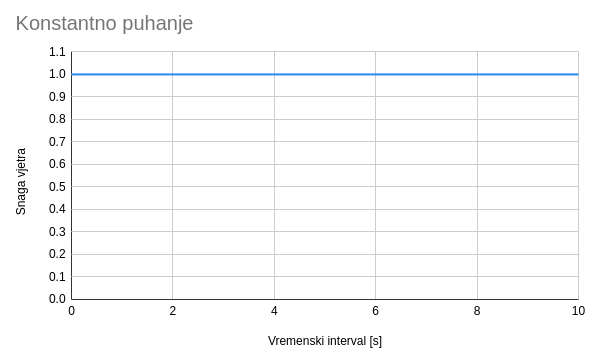
\includegraphics[width=0.8\textwidth]{img/43-1}
	\caption{Funkcija konstantog puhanja vjetra uz parametar snage 1}
	\label{fig:43-1}
\end{figure}

\paragraph{}
Puhanje u naletima vjetra jedan je od dinamičkih načina puhanja. Ovaj vjetar naivno modelira 
vjetre poput udara bure. Naivno modelira jer radi pretpostavku da vjetar potpuno stane 
između svakog udara. Na ovaj model utječe i parametar frekvencije. Na slici \ref{fig:43-2} 
prikazan je graf jednog takvog vjetra.

\begin{figure}[h]
	\centering
	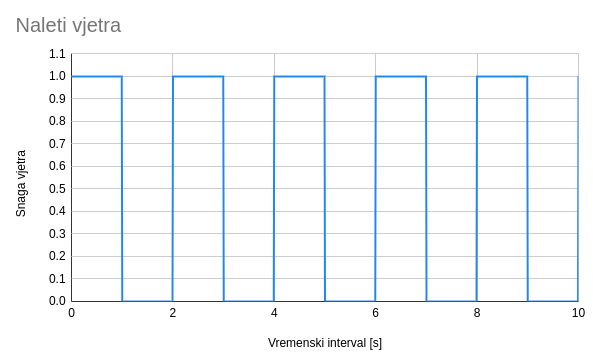
\includegraphics[width=0.8\textwidth]{img/43-2}
	\caption{Funkcija vjetra u udarima uz parametar snage 1 i frekvencije 0.5}
	\label{fig:43-2}
\end{figure}

\paragraph{}
Puhanje u valovima najrealističnija je simulacija vjetra. U ovakvom načinu vjetar polako 
puše sve većom snagom oko nazivne snage i kada dostigne dvostruku nazivnu snagu krene lagano 
opadati. Ovo je modelirano sinusoidom oko nazivne snage vjetra s amplitudom snage vjetra.
Na ovaj model također utječe parametar frekvencije.

\begin{figure}[h]
	\centering
	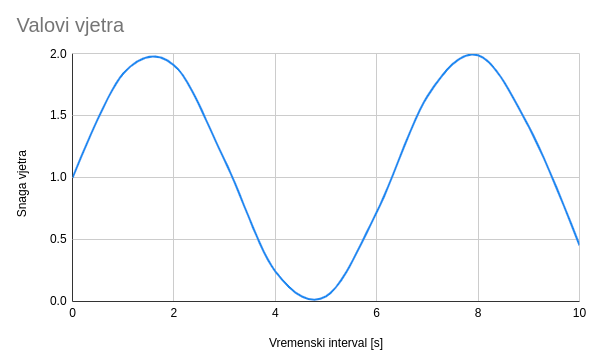
\includegraphics[width=0.8\textwidth]{img/43-3}
	\caption{Funkcija vjetra u valovima uz parametar snage 1 i frekvencije 0.16}
	\label{fig:43-3}
\end{figure}

\paragraph{}
Utjecaj parametara na simulaciju opisan je u poglavlju \ref{physics_model_eval}.

\chapter{Ocjena rezultata}
\section{Realističnost prikaza}
\paragraph{}
Realističnost prikaza nije bila primarna zadaća ovog rada. Generirane biljke ne 
izgledaju osobito prirodno bez obzira na razinu detalja kojom su generirane. Primjer 
generiranih biljaka vidljiv je na slici \ref{fig:51-1}.
\begin{figure}[h]
	\centering
	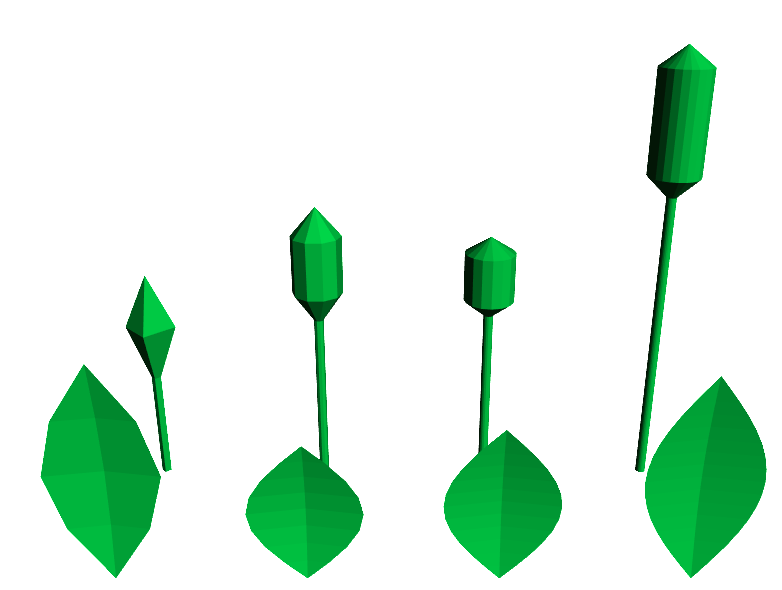
\includegraphics[width=0.8\textwidth]{img/51-1}
	\caption{Prikaz modela u različitoj razini detalja}
	\label{fig:51-1}
\end{figure}
\paragraph{}
Prvi razlog je primjena konstantnog sjenčanja poligona. U ovakvom načinu 
sjenčanja, normale za pojedine vrhove računamo kao normalu površine (poligona)
kojeg oni zatvaraju. Izračunata vrijednost normale se pripisuje svim vrhovima
poligona. Korištenjem konstantnog sjenčanja poligona postižemo jasno 
vidljivu granicu između pojedinih površina. Takav način prikaza, osim što je
vrlo brz u izvođenju, znatno je olakšao razvoj prezentiranog programskog 
rješenja jer daje programeru jasan uvid u poziciju pojedinih vrhova na ekranu
i njihovo ponašanje. 

\paragraph{}
Bez obzira na prednosti u razvoju koje ovakav pristup implicira, prikazani 
modeli izgledaju umjetno i izrazito su pravilni. Pravilnost modela je najveći
uzrok neprirodnog izgleda generiranih modela, jer na biljkama rijetko očekujemo
savršenu simetriju oko geometrijskih osi.
\paragraph{}
Drugi razlog je nedostatak detalja na generiranim modelima biljaka. Ovaj razlog 
dodatno naglašava pravilnost biljaka i smanjuje osjećaj realnosti prikaza.
Smanjenje broja detalja donijelo je iste prednosti kao i prethodni pristup - 
lakši razvoj i bolje performanse po cijenu realističnosti prikaza.
\paragraph{}
Treći razlog je izolacija prikaza. Biljke su prikazane kao centralni i jedini 
dio prikaza. Ovakav vakuum u prostoru dodatno naglašava oba prije spomenuta 
problema. Nedostatak simulacije atmosfere (prašina, distorzija zraka svjetlosti 
kao posljedica vlage u zraku itd.) uzrokuje dojam statičnosti biljaka bez
obzira na animirani prikaz ponašanja vjetra. Izostavak navedenih značajki, kao
i prethodna pojednostavljenja, olakšalo je razvoj programskog rješenja i 
oslobodilo vrijeme za ostvarenje kvalitetnije simulacije vjetra.

\subsection{Mogućnosti poboljšanja}
\paragraph{}
Problem sjenčanja može se riješiti primjenom nekog drugog načina sjenčanja 
modela korištenjem Gouraudovog sjenčanja. Korištenje ove metode 
sjenčanja eliminiralo bi vidljivost pojedinih vrhova na modelu i interpolacijom
između vrhova osiguralo gladak prijelaz između osjenčanih i ne osjenčanih 
dijelova modela. 
\paragraph{}
Biljke u stvarnosti rijetko imaju ikakve oštre bridove između svojih strana i 
zaglađivanje intenziteta osvjetljenja Gouraudovog sjenčanja između vrhova bi 
rezultiralo uvjerljivijim prikazom kod modela generiranih u većoj razini 
detalja. Kod modela generiranih manjom razinom detalja, rubovi samog modela bi
ostali oštri iako je model zaglađen. Sraz između rubova i unutrašnjosti modela
može uzrokovati smanjenje realističnosti prikaza.
\paragraph{}
Dodavanje malih varijacija kod generiranja modela poboljšalo bi realističnost 
prikaza. Mali istupi točaka od centra simetrije dali bi biljkama prirodniji
izgled uvođenjem nesavršenosti i raznovrsnosti biljaka. Osim dodavanja istupa
u poziciji točaka u modelu, istupi se mogu dodati i na boje pojedinih površina,
gdje bi neke površine bile više ili manje intenzivne boje od drugih. Dodavanje
boja u kombinaciji s Gouraudovim sjenčanjem dodatno bi pojačalo realističnost
prikaza.
\paragraph{}
Dodavanje varijacija je programski izrazito jednostavno za implementaciju ali
uzrokuje usporenje izvođenja, jer se svaki model zbog svoje unikatnosti mora
preslikati u memoriju grafičke kartice umjesto korištenja istog modela za sve 
biljke iste vrste. Kompromis se može postići na sredini - imati limitiran broj 
različitih modela iste vrste biljke koji se nasumično odabere za svaku biljku 
prilikom njenog kreiranja.
\paragraph{}
Dodavanje atmosferskih efekata na simulaciju bi uvelike pomoglo realističnosti
prikaza i dojmu živosti biljaka. Ovaj pristup rješavanju nerealističnosti 
prikaza je najkompleksniji od ponuđenih alternativa i zahtjeva razvoj nekolicine 
popratnih sustava, ali dao bi najveći doprinos realističnosti prikaza. Primjeri 
popratnih sustava koje je potrebno razviti uključuju: sustav ukrasnih čestica, 
sustav efekata nakon iscrtavanja (engl. \textit{post-processing effects}) i 
druge. 

\section{Realističnost fizičke simulacije} \label{physics_model_eval}
\paragraph{}
Bez obzira na jednostavnost implementacije fizičke simulacije i snažne
pretpostavke uključene u nju, fizička simulacija daje zadovoljavajuće rezultate.
Ponašanje prati stvarno prirodno gibanje u tri dimenzije i ne potiče osjećaj 
umjetnosti ili ograničenosti prolaskom kroz prostor. Simulacija dobro modelira
utjecaj visine biljke na njezinu simulaciju na vjetru. 
\paragraph{}
Na udarima vjetra visoke biljke rade velike i snažne zamahe i polagano gube 
energiju za nastavak daljnjeg osciliranja. Niske biljke rade kraće zamahe ali 
većom frekvencijom.
\paragraph{}
Kod konstantnog puhanja, biljke osciliraju prema točki konvergencije sile 
puhanja, sile teže i sila otpora unutar stabljike. Visoke biljke očekivano imaju veću 
amplitudu i manju frekvenciju oko te točke od niskih biljaka.
\paragraph{}
Puhanje s naletima vjetra također daje realistične rezultate. Niske biljke u 
naletu vjetra se brzo poravnavaju prema točki konvergencije i osciliraju oko 
nje, a po prestanku puhanja osciliraju oko centra ravnoteže velikom 
frekvencijom. Visoke biljke imaju veću tromost i rade veće oscilacije oko točke
konvergencije vjetra i otpora biljke prilikom naleta vjetra. Kad vjetar 
prestane, naprave manje oscilacija oko centra ravnoteže prije nego vjetar 
ponovno počne.
\begin{figure}[h]
	\centering
	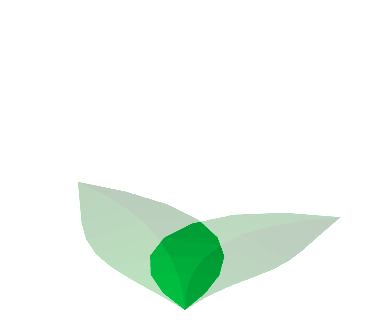
\includegraphics[width=0.4\textwidth]{img/52-1}
	\caption{Kaotično ponašanje niske biljke prilikom vjetra u valovima}
	\label{fig:52-1}
\end{figure}
\paragraph{}
Kad je simulacija vjetra realistična (takva da vjetar dolazi i prolazi u 
valovima - postepeno raste u snazi, i nakon toga postepeno opada u snazi) 
također imamo realističnu simulaciju. Visoke biljke održavaju smjer i neprestano 
osciliraju prema središtu između točaka centra ravnoteže otpora biljke, i 
konvergentne točke sile vjetra, ravnoteže i unutarnjeg otpora biljke. Niske 
biljke kod ovakvog vjetra djeluju kaotično i osciliraju velikom frekvencijom i 
amplitudom, sa središtem oscilacije koji vidno varira između konvergentne točke 
i centra ravnoteže biljke. Razlika u ponašanju je vidljiva na slikama \ref{fig:52-1} i \ref{fig:52-2}
\begin{figure}[h]
	\centering
	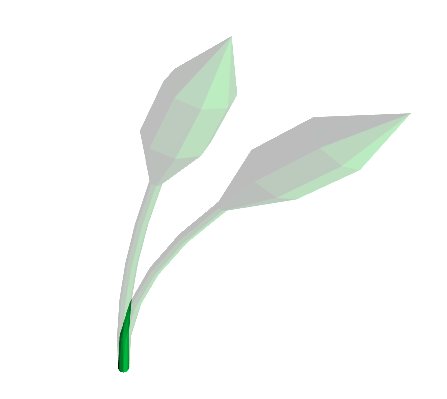
\includegraphics[width=0.4\textwidth]{img/52-2}
	\caption{Stabilno ponašanje visoke biljke prilikom vjetra u valovima}
	\label{fig:52-2}
\end{figure}

\subsection{Poboljšanje realističnosti simulacije}
\paragraph{}
Još realističnija simulacija se može postići dodavanjem većeg broja zglobova u
fizički kostur biljke. Dodavanjem većeg broja zglobova dobili bi mogućnost 
simulacije pregiba u stabljici biljke. U prirodi kod jednostavnih biljaka ovaj 
fenomen nije uvijek jasno vidljiv, ali možemo ga uočiti kad je vjetar u 
rezonantnoj frekvenciji sa stabljikom biljke.
\paragraph{}
Dodatnu kontrolu možemo postići dodavanjem težina pojedinim zglobovima. Tako da 
na neke dijelove kostura vjetar ima jači utjecaj nego na druge. Primjer takve 
biljke je zvončić, kod kojeg je utjecaj vjetra puno jasnije vidljiv na cvijetu 
nego na stabljici biljke.

\section{Brzina izvođenja}
\paragraph{}
Brzina izvođenja linearno opada s brojem simuliranih biljaka. Najveći utjecaj na 
brzinu izvođenja ima fizička simulacija. Generiranje biljaka se odvija na samom 
početku i nema nikakvog utjecaja na brzinu izvođenja nakon početnog perioda 
generiranja. Iscrtavanje je zbog jednostavnosti prikaza vrlo jeftino i usporava
izvođenje tek na velikom broju biljaka ili na vrlo visokoj razini detalja. Graf trajanja 
vremenskog koraka vidljiv je na \ref{fig:53-1}.

\begin{figure}[h]
	\centering
	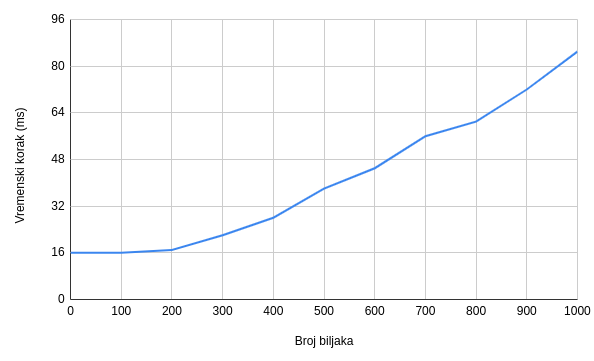
\includegraphics[width=0.95\textwidth]{img/53-1}
	\caption{Trajanje vremenskog koraka u ovisnosti o broju biljaka u simulaciji}
	\label{fig:53-1}
\end{figure}

\subsection{Pristupi poboljšanju brzine izvođenja}
\paragraph{}
Fizička simulacija ima najveći utjecaj na brzinu izvođenja pa su prijedlozi za 
ubrzanje programskog rješenja fokusirani na taj dio.
\subsubsection{Paralelno izvođenje fizičke simulacije}
\paragraph{}
Trenutna programska implementacija u obzir uzima i kolizije samih biljaka. 
Fizička simulacija se odvija slijedno za svaku od biljaka i eventualni dodir 
nakon simulacije neke od narednih biljaka može imati utjecaj na onu prvu. Ako
ne marimo za interakciju između samih biljaka i odlučimo je zanemariti, 
jednostavan način za ubrzanje fizičke simulacije je paralelizam. Na \ref{fig:531-1} je 
prikazan dijagram slijednog i paralelnog izvođenja (na dvije dretve) i vidljivo je da 
paralelni primjer završava u dva koraka dok slijedni algoritam završava u jednom koraku.

\begin{figure}[h]
	\centering
	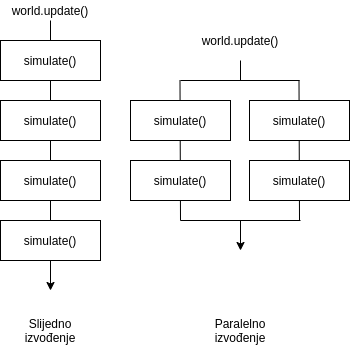
\includegraphics[width=0.7\textwidth]{img/531-1}
	\caption{Dijagram slijednog i paralelnog izvođenja}
	\label{fig:531-1}
\end{figure}
\paragraph{}
Na ovaj način svaka biljka (ili grupa biljaka) može imati svoj fizički procesor 
koji će se brinuti o njezinoj simulaciji i cijeli proces se završava u manje 
koraka.

\subsubsection{Smanjenje rezolucije simulacije i zaglađivanje rezultata}
\paragraph{}
Brzinu izvođenja možemo i povećati tako da ne ažuriramo fizičku simulaciju 
biljke u svakom koraku. Kod ovakvog pristupa stanje svake biljke izračunavamo 
nakon nekoliko koraka umjesto na svakom, a rezultate u međukoracima zagladimo.
U primjeru \ref{fig:531-2} vidimo slijed simulacije jedne biljke kroz vremenske 
korake. Prilikom simulacije trebamo osigurati da je vremenski razmak za koji 
simuliramo točno onoliko koraka koliko će trajati do sljedeće simulacije i to 
uzrokuje smanjenje rezolucije simulacije. Ako bi vremenski korak simulacije 
ostao jednak kao da simuliramo biljku u svakom simulacija bi se odvijala 
usporeno.
\paragraph{}
Bitno je ostvariti da se nikad istovremeno ne simuliraju i zaglađuju svi modeli 
nego da je postupak naizmjeničan. Za primjer dvije biljke, dok se jedna 
biljka simulira druga se zaglađuje i obratno.
\begin{figure}[h]
	\centering
	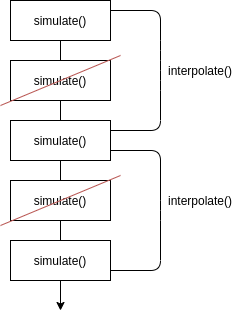
\includegraphics[width=0.5\textwidth]{img/531-2}
	\caption{Dijagram simulacije sa zaglađivanjem}
	\label{fig:531-2}
\end{figure}
\paragraph{}
Problem kod ovakvog pristupa je kašnjenje prikaza nad stvarnim stanjem fizičke 
simulacije. Fizička simulacija je uvijek barem jedan korak ispred prikaza. Ovo 
može uzrokovati naizgledno podrhtavanje ako želimo zadržati simulaciju 
interakcija između biljaka, a biljka se pomaknula nakon što je dobivena zadnja 
točka za interpolaciju. Ako ne marimo za interakciju između biljaka, ovaj 
problem možemo zanemariti. Iako će animacija i dalje kasniti za stvarnim 
fizičkim stanjem, promatraču to neće biti vidljivo.
\subsubsection{Izračunavanje sličnosti modela i grupiranje izračuna}
\paragraph{}
Ako nam nije bitna interakcija između biljaka i želimo drastično smanjiti utjecaj 
fizičke simulacije na brzinu izvođenja možemo izdvojiti prototipne biljke iz simulacije i 
simulirati samo njih. Sve ostale biljke, ovisno o sličnosti će koristiti podatke simulacije 
te biljke kao svoje. Primjer takvog sustava vidljiv je na slici \ref{fig:531-3}
\begin{figure}[h]
	\centering
	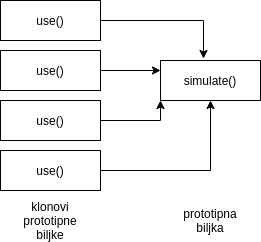
\includegraphics[width=0.5\textwidth]{img/531-3}
	\caption{Dijagram simulacije sa grupiranjem}
	\label{fig:531-3}
\end{figure}
\paragraph{}
Na ovaj način potrebno je simulirati samo nekoliko biljaka umjesto svih ali ovakav pristup 
će rezultirati time da simulacija izgleda nerealistično jer će sličnosti između ponašanja 
biljaka biti identične u isto vrijeme i na istim uvjetima što narušava dojam realizma. 
Potencijalno rješenje ovog problema je da kod nekih biljaka unesemo kašnjenje nad 
prototipnom biljkom. Tako smo eliminirali problem dojma da se sve ponavlja, ali smo 
uveli problem da simulacija ne djeluje toliko responzivno.

\chapter{Zaključak}
\paragraph{}
Generiranje i simulacija trave i niskog raslinja je moguća, ali i takav način izrade 
modela iziskuje veliku količinu vremena. Nakon početnog uloženog vremena, proces same izrade 
je ubrzan ali zahtjeva daljnji razvoj infrastrukture jer je za svaku novu karakteristiku 
neke biljke potrebno vrijeme kako bi se ona matematički opisala i razvila. Rezultati 
dobiveni ovom tehnikom mogu izgledati siromašno i potrebno je uložiti dodatan trud kako bi 
se takvi modeli efektivno iskoristili.

\paragraph{}
Ovakav model generiranja i simuliranja modela bi ipak, uz neka poboljšanja, mogao biti 
isplativ u izrazito velikim igrama ili kao rješenje koje bi se koristilo u više igara. 
Ulaganjem vremena u ovakav sustav generiranja modela moguće je dostignuti razinu gdje je 
gotovo svaku biljku moguće vrlo jednostavno opisati s par pravila. Model simulacije vjetra 
koji je istražen je jednostavan i uz dodatne optimizacije bi se efektivno mogao koristiti u 
igrama, čak i sa ručno modeliranim modelima biljaka.

\nocite{*}
\bibliography{diplomski}
\bibliographystyle{fer}

\listoffigures
\lstlistoflistings
\addcontentsline{toc}{chapter}{Popis isječaka koda}

\begin{sazetak}
Proceduralno generiranje modela trave i niskog raslinja te simulacija njihovog ponašanja na 
različitim atmosferskim utjecajima je kompleksan matematički problem. Promatranjem izgleda 
biljaka i njihovog ponašanja moguće je uočiti pravilnosti. Korištenjem tih pravilnosti kao 
pretpostavki u izgradnji modela prikaza i fizičkog modela simulacije, moguće je vrlo 
jednostavnim matematičkim konstrukcijama doći do modela koji vjerno opisuje stvarno 
ponašanje. U ovom radu su istražene i implementirane tehnike za generiranje 3D modela trave 
i niskog raslinja. Ponuđen je razvojni okvir za izradu proizvoljnih 3D modela te osnovni 
sustav simulacije vjetra. Ocijenjeni su i prezentirani rezultati. Istražene su neke 
mogućnosti za nastavak istraživanja.

\kljucnerijeci{proceduralno generiranje, simulacija vjetra, omatanje modela, fizička simulacija}
\end{sazetak}

% TODO: Navedite naslov na engleskom jeziku.
\engtitle{Procedural generation of grass and low vegetation}
\begin{abstract}
Procedural generation of grass and low vegetation models, with simulated behavior under 
different atmospheric conditions is a complex mathematical problem. By observing plants it 
is possible to deduct some regularities about their appearance and behavior. Using those 
regularities as assumptions while building graphics and physics model it is possible to 
achieve level of realism with just simple mathematical constructions. This paper researched 
and implemented some of the techniques used for generating 3D models of grass and low 
vegetation. It offers a framework for creating a wide range of different plants and basic 
system for wind simulation. Results were measured and are presented. Paper explored some of the possibilities for the continuation of research.

\keywords{procedural generation, wind simulation, model skinning, physics simulation}
\end{abstract}

\end{document}
